\chapter{Capitolo 3: Albero Evolutivo}
Una delle sfide più importanti della bioinformatica, nonché l'obiettivo principale della filogenetica, è la costruzione degli alberi evolutivi.
\newline
Ricordando la definizione di albero, ovvero un grafo non orientato connesso e aciclico \cite{algoritmiEStruttureDati2}, \textit{L'albero evolutivo} o \textit{albero filogenetico} è un diagramma che rappresenta le relazioni evolutive tra i vari organismi \cite{buildingaphylogenictree}. La sua peculiarità consiste nel poterli costruire in base a dati genetici, genomici o morfologici, affinché si possano descrivere le relazioni che vi sono tra organismi viventi oppure tra specie estinte e specie viventi.
\newline
TODO: SISTEMARE!!!
\newline
\newline
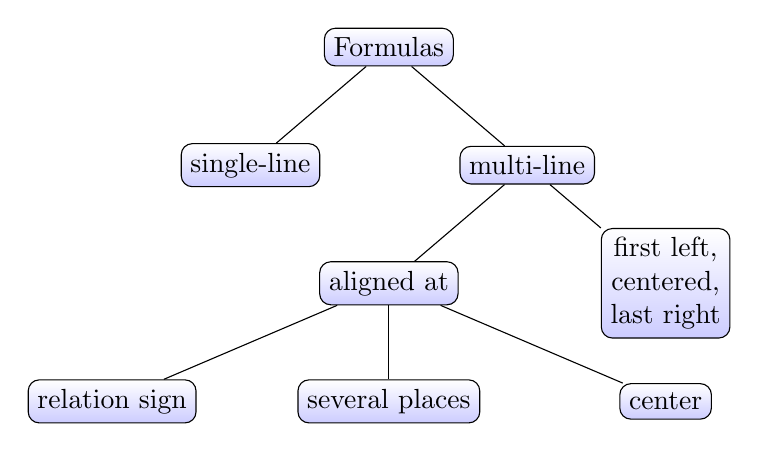
\begin{tikzpicture}[sibling distance=10em,
  every node/.style = {shape=rectangle, rounded corners,
    draw, align=center,
    top color=white, bottom color=blue!20}]]
  \node {Formulas}
    child { node {single-line} }
    child { node {multi-line}
      child { node {aligned at}
        child { node {relation sign} }
        child { node {several places} }
        child { node {center} } }
      child { node {first left,\\centered,\\last right} } };
\end{tikzpicture}
\newpage
test bla bla bla testtest bla bla bla testtest bla bla bla testtest bla bla bla testtest bla bla bla testtest bla bla bla testtest bla bla bla testtest bla bla bla test
\newline
\begin{center}
\begin{forest}
for tree={circle,draw, l sep=32pt, s sep=33pt}
[k,red 
    [z,edge label={node[midway,left] {5}}
      [y,edge label={node[midway,left] {10}} ] 
      [l,edge label={node[midway,left] {12}}] 
      [m,edge label={node[midway,right] {7}}]
    ]
    [u,edge label={node[midway,right] {2}}
      [f,edge label={node[midway,left] {1}}] 
      [h,edge label={node[midway,left] {18}}] 
      [p,edge label={node[midway,right] {20}}]
  ] 
]
\end{forest}
\end{center}
test bla bla bla testtest bla bla bla testtest bla bla bla testtest bla bla bla testtest bla bla bla testtest bla bla bla testtest bla bla bla test





\newpage
Ordine dei capitoli:
\begin{itemize}
	\item Cap 3: alberi evolutivi;
	\item Cap 4: albero additivo;
	\item Cap 5: UPGMA (Unweighted Pair Group Method with Arithmetic Mean)
	\item cap 6: NEIGHBORJOINING
\end{itemize}

